\chapter{Ideal Work-cell}\label{IdealWorkCell}

\begin{figure}[h]
    \centering
    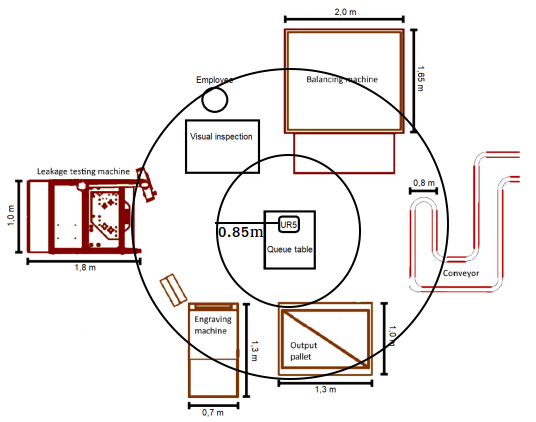
\includegraphics[width=9cm]{Design/Work_cell_3.png}
    \caption{work-cell with measurements and reach}
    \label{fig:workcellMR}
\end{figure}

When looking at \ref{fig:workcellMR}, a systematic work-cell is presented. But the important thing of a work-cell is its flow.\\
Here is some sections about what is needed of the ideal work-cell.

\section{Dexterous workspace}

The workspace which a manipulator works within can be described as a radius which the point of the end-effector can reach.\\
The Dexterous workspace is a more intelligent way of the robot to decide which points in arbitrary orientation, can be reached \cite{Dexterous}.\\
The reason that the dexterous workspace is considered a solution to the work-cell, is that the kinematic restrains can be included, so that the trajectories of the manipulator wont freeze or go in lock down.\\


\section{Safety}

To keep the production safe and manageable, some of the safety devices are chosen:

\begin{itemize}
    \item Light Curtain
    \item Lidar
\end{itemize}

The light curtain provides a signal when the curtain is broken, see \ref{SafetyDevices}.\\
This will be used to send a signal to the UR5 to either stop or slow down the production, so a person safely can enter the cell, without getting serious damages.\\

The Lidar is commonly used in production, see \ref{SafetyDevices}.
This threshold can be used to measure when a person enters the hazardous work area of the UR5.\\
All of the above is a must since the UR5 is carrying a metal rotor with sharp edges, so the person wont be gauged.\\

\subsection{Safety Requirements}

The most important solution for the safety of the work-cell, is the ISO 10218-2:2011, see \ref{ISO2}.\\
When installing a new robot for a production line, some standards is required. These standards of the ISO can present which of the areas needed to be acted upon.\\

\section{Placement Sensors}

To ensure the work-flow some intelligent placement sensors must be implemented. Some of the possible solutions are chosen:\\

\begin{itemize}
    \item Lidar
    \item Photocell sensors
    \item Depth sensing camera
\end{itemize}

The Lidar is a sensor that gives a 3D view, and can be used for the robot to tell the different object apart, and give an overview of the work-cell, see \ref{ref:PlacementS}.\\
These signals can be used for the cobot to get a better work-flow and also determine objects from each other.\\

The photocell sensors can be used for a quicker work-flow, since it will detect the rotors when they are in the correct place to be picked up, see \ref{ref:PlacementS}.\\

Depth sensing cameras can determine the distance from end-effector to the desired object, see \ref{ref:PlacementS}. This can be used to derive the distance from the certain machine where the rotor has to be placed.\\

\chapter{Ideal Robot}\label{IdealRobot}

The ideal robot to have inside the work-cell, is intelligent, fast and can decide the next trajectory without any hesitation. Its size is optimized to fit the given case, to work at the most effective speed possible.\\

\section{Optimal speed}

The robot has 7 tasks it needs to complete within 26 seconds. This means that the slowest possible speed it has to have per translation to other machines, while delivering the rotor, is 26 divided by 7, which will give the manipulator 3.7142 seconds to carry out the task.\\
Taking the visual inspection in consideration, the number has to be lower when translating from the machines. The person inspecting might need something close to 5 seconds. Taking that into consideration a new formula for the speed of the cobot can be found.\\

\begin{equation}
    26 = 5 + 6 \times b \Rightarrow b = \frac{21}{6}\\
\end{equation}

\begin{equation}
    b = \frac{21}{6} \Rightarrow b = \frac{7}{2}\\
\end{equation}

\begin{equation}
    b = \frac{7}{2} \Leftrightarrow  b = 3.5 sec\\
\end{equation}

\newpage
5 seconds in one station means that the other stations needs to be cut down with 0.2 seconds each.\\
So the optimal speed for translations would be 3.5 seconds.\\

\section{optimal reach}

The manipulator must be able to reach all machines, without having to move its base. Given the work-cell design, this means the robot will need a reach of 2 meters. \\
\begin{figure}[h]
    \centering
    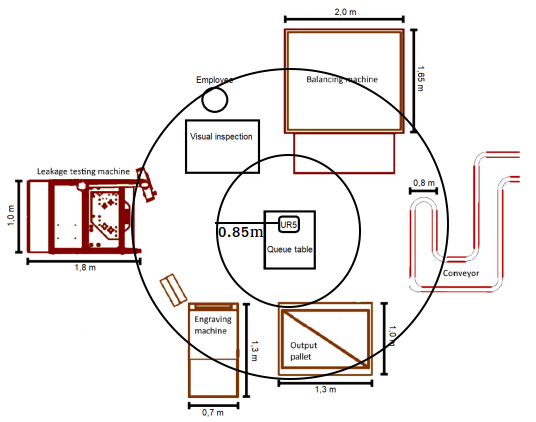
\includegraphics[width=8cm]{Design/Work_cell_3.png}
    \caption{Work-cell with measurements and reach}
    \label{fig:workcell}
\end{figure}

This optimal reach could also be accomplished by changing the setup to use 2 manipulators, thereby halving the required reach. By doing it this way, the 2 robots would only need one place where their reach overlap, so they can both pick and place the rotors on a buffer table. This would also require additional safety, that should prevent the to robots from hitting each other.\\

\begin{figure}[h]
    \centering
    \includegraphics[width=8cm]{}
    \caption{Work-cell design with 2 robots}
    \label{fig:workscell2arms}
\end{figure}

\section{optimal sensors}

The robot should be able to identify humans, and collisions must be risk free, and not disrupt the work-flow. Optimally, the robot should also be able to identify what object it is holding, and if it is damaged or not. Additionally, the robot must be able to place the rotors correctly in the machines, using a depth sensing camera. \ref{depthcam}\\
The robot should be able to register whether or not it has picked up a rotor. This can be done by using a pressure sensor.\\ 

\subsection{max payload}

The robot must be able to lift the L40 rotor given in the case, which weighs 645 grams. The end-effector must also be able to grab it, without the risk of dropping it. The rotor is 190mm long, and 90mm wide at its widest point. The manipulator must also be able to support the[width=8cm] weight when the arm is fully stretcworkscell2arms















